\hypertarget{dl_8c}{\section{dl.\+c File Reference}
\label{dl_8c}\index{dl.\+c@{dl.\+c}}
}


Loading modules under linux.  


{\ttfamily \#include $<$kdbconfig.\+h$>$}\\*
{\ttfamily \#include $<$dlfcn.\+h$>$}\\*
{\ttfamily \#include $<$kdberrors.\+h$>$}\\*
{\ttfamily \#include $<$kdbmodule.\+h$>$}\\*
{\ttfamily \#include $<$stdlib.\+h$>$}\\*
{\ttfamily \#include $<$string.\+h$>$}\\*
Include dependency graph for dl.\+c\+:
\nopagebreak
\begin{figure}[H]
\begin{center}
\leavevmode
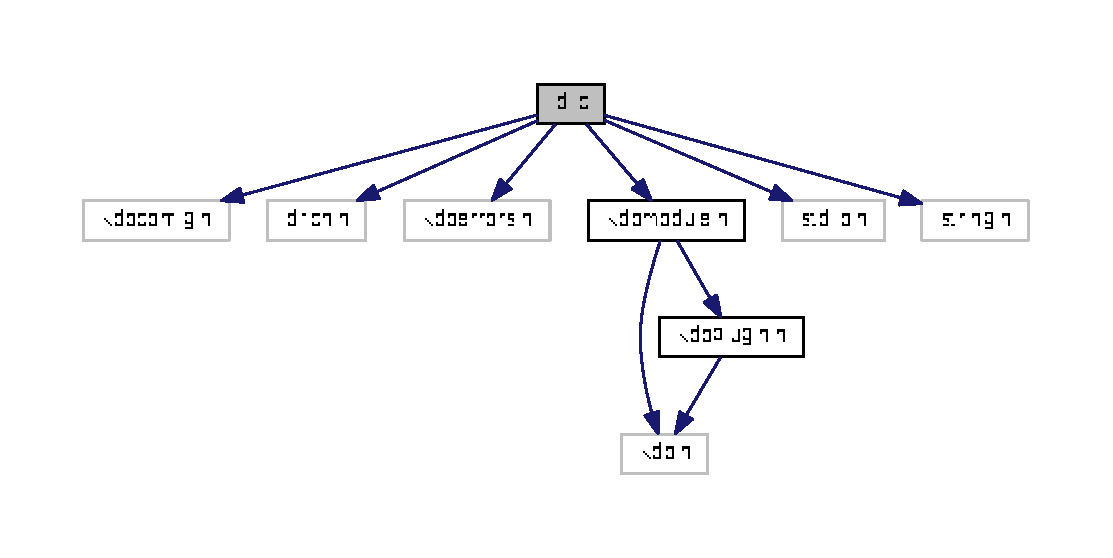
\includegraphics[width=350pt]{dl_8c__incl}
\end{center}
\end{figure}


\subsection{Detailed Description}
Loading modules under linux. 

\begin{DoxyCopyright}{Copyright}
B\+S\+D License (see doc/\+C\+O\+P\+Y\+I\+N\+G or \href{http://www.libelektra.org}{\tt http\+://www.\+libelektra.\+org})
\end{DoxyCopyright}
The name of the module will be libname. A .so will be appended. This file will be loaded.

The path were the plugins are located, e.\+g. /usr/src/elektra need to be added with L\+D\+\_\+\+L\+I\+B\+R\+A\+R\+Y\+\_\+\+P\+A\+T\+H.

The reason is that only L\+D\+\_\+\+L\+I\+B\+R\+A\+R\+Y\+\_\+\+P\+A\+T\+H also loads libraries which are seen by symlink only. That feature is needed for libelektra-\/default.

The buildsystem makes sure that dlfcn.\+h exists. 